\section{Контрольная работа \textnumero2}

\subsection{Задача \textnumero1}
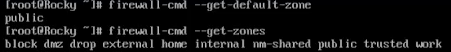
\includegraphics{1.png}
\subsubsection{Решение}
Модель естесственного роста выпуска продукции при убывающей цене:
\begin{equation} \label{eq:model}
	y'(t) = mp(t)ly(t)
\end{equation}
где: \\
$m$ -- норма инвестиции, $p$ -- цена, $\frac{1}{l}$ -- норма акселерации, а $y(t)$ -- выпуск продукции, реализованный к моменту времени $t$ \\
Значит:
\begin{gather*}
	y'(t) = \frac{1}{2} \times (2 - y(t)) \times 2 \times y(t) \\
	y'(t) = (2 - y(t))y(t) \\
\end{gather*}

\newpage
\subsection{Задача \textnumero2}
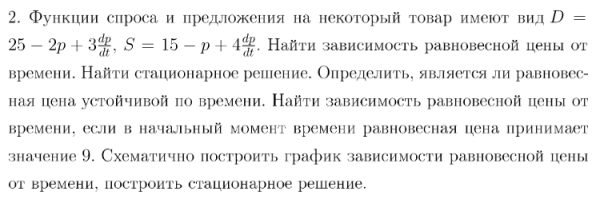
\includegraphics{2.png}
\subsubsection{Решение}
\begin{gather*}
	D(p^*) = S(p^*), p^* \textup{ --- равновестаная цена} \\
	25 - 2p + 3p' = 15 - p + 4p' \\
	p' + p = 10 \\
\end{gather*}

\newpage
\subsection{Задача \textnumero3}
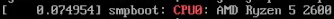
\includegraphics{3.png}
